\documentclass[conference]{IEEEtran}

\usepackage{cite}
\usepackage{amsmath}
\usepackage{graphicx}
\usepackage{booktabs}
\usepackage{array}
\usepackage{url}

\title{Stock Price Forecasting Across Prediction Horizons and Volatility Regimes}

\author{\IEEEauthorblockN{Xinzhuo Li}
\IEEEauthorblockA{STATS 507 Final Project}}

\begin{document}

\maketitle

\begin{abstract}
Forecasting financial time series is difficult because market prices are noisy, non-stationary, and highly sensitive to volatility. This project studies how predictive performance changes across forecast horizons and volatility regimes using a public Yahoo Finance daily price dataset spanning May 2018 to April 2023. After cleaning, the dataset contains 1,258 observations with open, high, low, close, adjusted close, and volume fields. Lagged prices, returns, rolling averages, rolling volatility, log-volume, and intraday range were used to construct a supervised learning dataset for three horizons: one day, three days, and seven days ahead. Four models were evaluated using chronological train/validation/test splits: a naive persistence baseline, linear regression, a validation-tuned random forest, and an LSTM network. Across all three horizons, the naive baseline achieved the lowest test RMSE, with values of 376.76, 655.81, and 977.89 for horizons 1, 3, and 7, respectively. Error increased substantially with longer horizons and under high-volatility conditions. A lightweight tuning step was added for the random forest, but the tuned model still did not outperform the simpler baselines. The results suggest that short-term price persistence remains difficult to beat in a small single-series setting, while more complex models require either richer features or more data to consistently outperform simple baselines.
\end{abstract}

Code, generated outputs, and the final report are available at \url{https://github.com/Xinzhuo-Li/stats507-final-project}.

\section{Introduction}
Stock price forecasting is a classic problem in data science because it combines practical importance with substantial modeling difficulty. Financial markets react to information quickly, and the resulting time series often exhibit non-stationarity, heteroskedasticity, and abrupt regime changes. These properties make it challenging for a model trained on historical data to generalize well to future observations. The efficient market view highlights why this task is difficult: if prices already incorporate available information, short-term prediction opportunities may be limited or unstable \cite{fama1970efficient}.

Even so, forecasting remains useful because model performance can vary across settings. In particular, predictive difficulty often changes with the forecast horizon and with market volatility. A one-day-ahead task may be dominated by local persistence, while a seven-day-ahead task may require broader pattern extraction. Likewise, highly volatile periods can weaken the stability of relationships learned during calmer periods.

This project investigates two main questions:
\begin{enumerate}
    \item How does forecasting accuracy change across one-day, three-day, and seven-day horizons?
    \item How does model performance differ between low- and high-volatility market conditions?
\end{enumerate}

To answer these questions, this study compares models with different levels of complexity, ranging from a naive persistence baseline to linear regression, random forest, and LSTM. The goal is not only to identify the strongest model, but also to understand when model complexity helps and when it does not.

\section{Related Work}
Research on financial prediction spans classical finance, machine learning, and deep learning. Fama's survey on efficient capital markets provides the theoretical foundation for why consistent excess predictability is hard to obtain in financial data \cite{fama1970efficient}. In practical forecasting tasks, however, researchers often still find that carefully designed features and models can provide useful short-term structure.

Traditional machine learning methods remain important because they can operate effectively on engineered tabular features. Random forests are especially attractive because they capture nonlinear interactions without requiring strong distributional assumptions \cite{breiman2001random}. In financial prediction settings, Patel et al. showed that machine learning approaches can improve stock and index movement prediction when technical features are prepared carefully \cite{patel2015stock}.

Deep learning methods target temporal dependency more directly. Hochreiter and Schmidhuber introduced the LSTM architecture to address long-range dependency learning in recurrent models \cite{hochreiter1997lstm}. In finance, Fischer and Krauss demonstrated that LSTM models can be competitive for market prediction tasks, especially when enough sequential structure is available for the model to learn \cite{fischer2018lstmfinance}. Motivated by this literature, the current project compares classical and sequence-based approaches within the same experimental pipeline.

\section{Method}
\subsection{Dataset}
The dataset is a public Yahoo Finance daily price file covering May 1, 2018 through April 28, 2023. After cleaning invalid rows and sorting chronologically, the final dataset contains 1,258 observations. The raw columns are \texttt{Open}, \texttt{High}, \texttt{Low}, \texttt{Close}, \texttt{Adj Close}, and \texttt{Volume}. The adjusted close price is used as the target variable because it is a standard total-return-aware price field for historical analysis.

\subsection{Problem Formulation}
Let $x_t$ denote the feature vector available at trading day $t$. For a forecast horizon $h \in \{1, 3, 7\}$, the prediction target is
\[
y_t^{(h)} = \text{AdjClose}_{t+h}.
\]
This creates three supervised learning tasks: predict the adjusted close one day, three days, and seven days into the future. The forecast origin in this project is the \emph{end of day} at time $t$, meaning that the full OHLCV record for day $t$ is assumed to be observed before making a forecast for $t+1$, $t+3$, or $t+7$. Under this setup, same-day close and adjusted close are valid inputs, but they also make persistence-style baselines especially strong.

\subsection{Feature Engineering}
The feature set combines raw prices with derived temporal statistics:
\begin{itemize}
    \item current-day open, high, low, close, adjusted close, and volume;
    \item daily return;
    \item log-volume;
    \item intraday range $(\text{High} - \text{Low}) / \text{Open}$;
    \item lagged adjusted close values for 1, 2, 3, 5, and 10 days;
    \item lagged daily returns for 1, 2, and 3 days;
    \item 5-day and 10-day rolling means of adjusted close;
    \item 5-day and 10-day rolling standard deviations of daily returns.
\end{itemize}

These features were chosen to capture local trend, momentum, and volatility effects while staying interpretable and consistent across models.

\subsection{Models}
Four models were evaluated:
\begin{itemize}
    \item \textbf{Naive baseline}: predicts the future adjusted close using the current adjusted close.
    \item \textbf{Linear regression}: a standardized linear model serving as an interpretable baseline.
    \item \textbf{Random forest}: a nonlinear ensemble model whose hyperparameters were selected with a validation-set grid search.
    \item \textbf{LSTM}: a sequence model with sequence length 20, hidden size 32, batch size 32, learning rate $10^{-3}$, and 40 epochs.
\end{itemize}

For preprocessing, linear regression used standardized inputs. Random forest was trained on the same tabular features without scaling. For the LSTM, input features were standardized using training-set means and standard deviations, and the target was standardized during training and transformed back to the original price scale at inference time.

\subsection{Evaluation Design}
The data were split chronologically into training, validation, and test sets using a 60\%/20\%/20\% ratio. This avoids look-ahead bias and better reflects real forecasting conditions. Model performance was measured using RMSE, MAE, $R^2$, and MAPE. MAPE was included as a scale-free supplementary metric; because the target is a positive price level far from zero throughout the sample, it remains interpretable here.

For the random forest, a lightweight tuning stage was added before test evaluation. The validation set was used to compare six candidate configurations over \texttt{n\_estimators}, \texttt{max\_depth}, and \texttt{min\_samples\_leaf}. The best settings were $(100, 8, 3)$ for the one-day horizon and $(300, 12, 1)$ for the three-day and seven-day horizons, where each tuple denotes \texttt{(n\_estimators, max\_depth, min\_samples\_leaf)}. After selecting the best configuration for each horizon, that tuned model was evaluated on the held-out test set.

For the LSTM, the training seed was fixed at 42, the optimizer was Adam, and the loss function was mean squared error. No early stopping was used; instead, a small fixed architecture was chosen to keep the comparison lightweight and reproducible.

To study market regimes, the 10-day rolling return standard deviation was used as a volatility indicator. The median training-set value served as the threshold separating low-volatility and high-volatility test observations. Each model was then re-evaluated within those two regimes.

\section{Results}
Table~\ref{tab:testmetrics} reports the main test-set results across all models and horizons after introducing random forest tuning. Two patterns are immediately clear. First, forecasting error increases sharply as the horizon grows from 1 day to 7 days. Second, the naive persistence baseline achieves the lowest overall RMSE at every horizon, with linear regression consistently ranking second.

\begin{table*}[t]
\centering
\caption{Test-set performance across prediction horizons.}
\label{tab:testmetrics}
\scriptsize
\begin{tabular}{c l r r r r}
\toprule
Horizon & Model & RMSE & MAE & $R^2$ & MAPE (\%) \\
\midrule
1 & Naive baseline & 376.76 & 285.06 & 0.9211 & 0.8846 \\
1 & Linear regression & 384.66 & 287.01 & 0.9178 & 0.8908 \\
1 & Random forest & 474.08 & 365.32 & 0.8751 & 1.1383 \\
1 & LSTM & 598.83 & 465.35 & 0.8123 & 1.4544 \\
\midrule
3 & Naive baseline & 655.81 & 517.94 & 0.7617 & 1.6111 \\
3 & Linear regression & 684.03 & 530.77 & 0.7407 & 1.6509 \\
3 & Random forest & 797.53 & 602.31 & 0.6476 & 1.8894 \\
3 & LSTM & 814.32 & 609.08 & 0.6542 & 1.9149 \\
\midrule
7 & Naive baseline & 977.89 & 773.32 & 0.4702 & 2.4098 \\
7 & Linear regression & 1040.18 & 815.02 & 0.4005 & 2.5322 \\
7 & LSTM & 1114.48 & 849.29 & 0.3522 & 2.6702 \\
7 & Random forest & 1317.82 & 1030.15 & 0.0378 & 3.2457 \\
\bottomrule
\end{tabular}
\end{table*}

Figure~\ref{fig:rmsehorizon} visualizes the RMSE comparison by horizon. The performance ranking is largely stable: naive baseline, linear regression, and then the two more flexible models. Importantly, the tuned random forest still does not outperform either naive persistence or linear regression. In this experiment, additional model flexibility does not translate into better generalization. More cautiously, the results suggest that the current adjusted close is already a strong near-term benchmark for this specific dataset and forecast definition.

\begin{figure}[t]
\centering
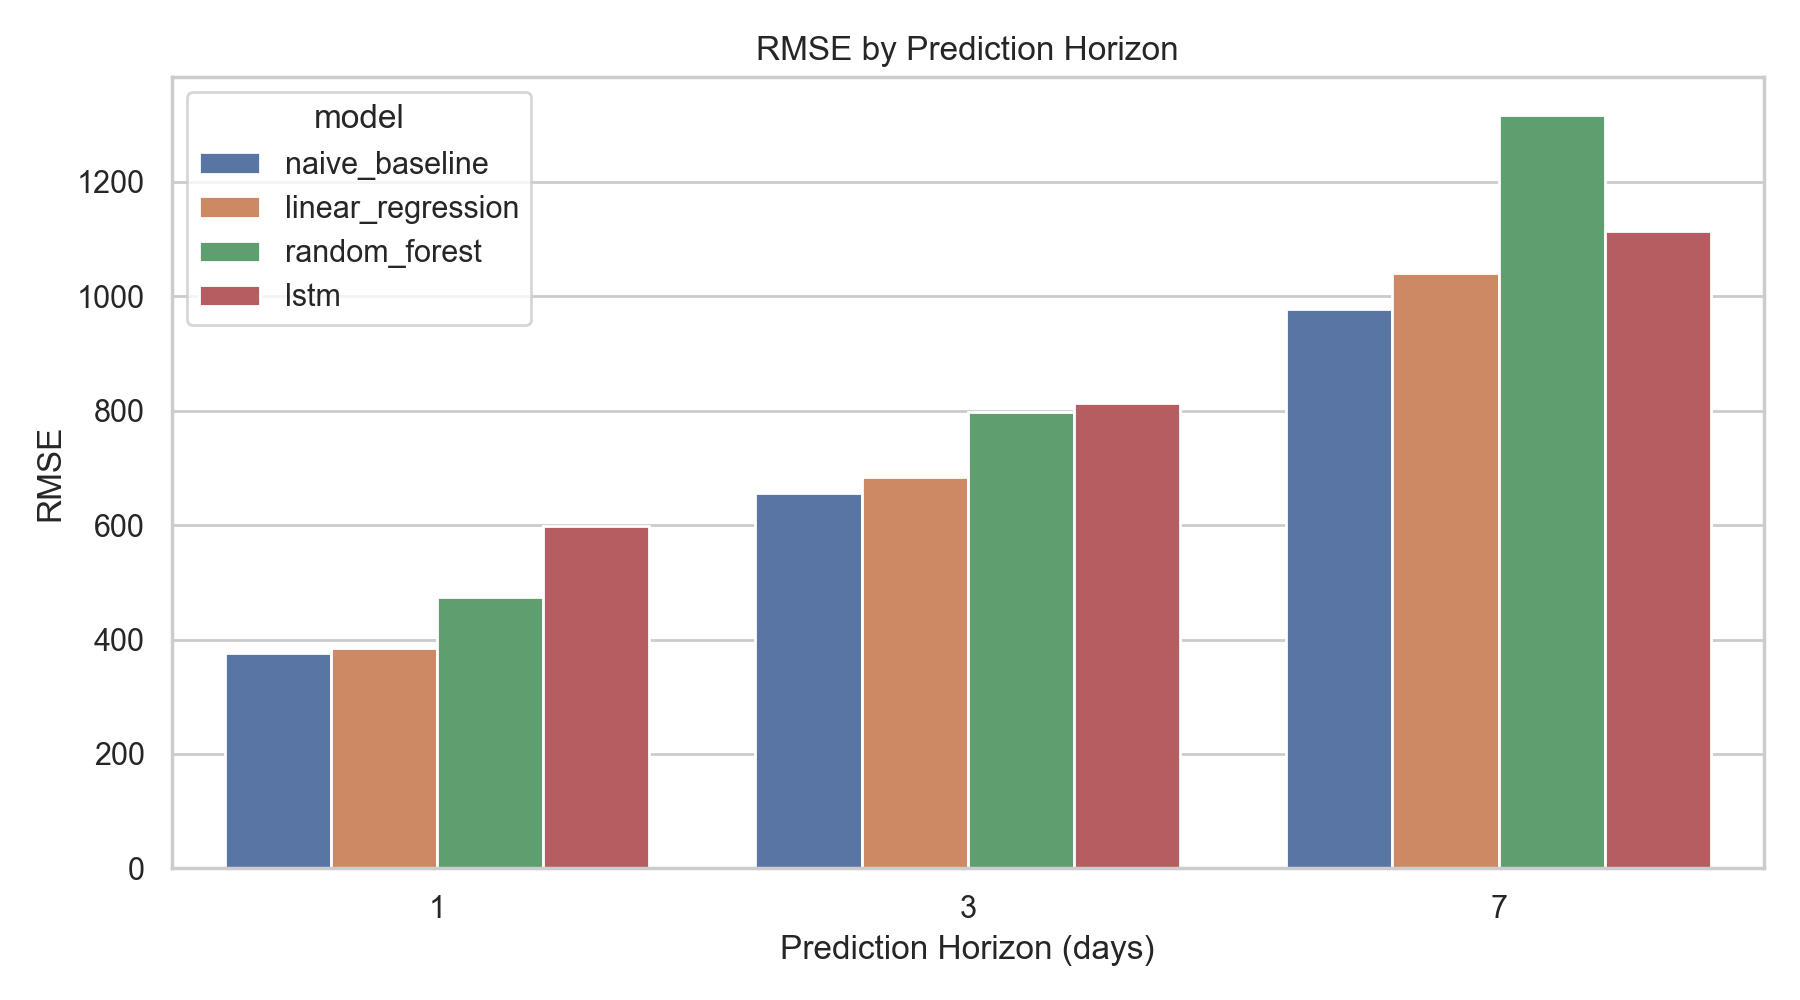
\includegraphics[width=\columnwidth]{../outputs/figures/rmse_by_horizon.png}
\caption{Test RMSE by prediction horizon and model.}
\label{fig:rmsehorizon}
\end{figure}

Volatility analysis adds a more nuanced view. Table~\ref{tab:regime} summarizes the best-performing model in each volatility regime. Under high volatility, the naive baseline is best at all three horizons. Under low volatility, more flexible models become competitive: random forest achieves the lowest RMSE for the one-day horizon, while LSTM is best for the three-day and seven-day horizons. These patterns should be interpreted cautiously because the low-volatility subsets are small, ranging from 32 to 38 test observations depending on horizon.

\begin{table}[t]
\centering
\caption{Best RMSE by volatility regime.}
\label{tab:regime}
\scriptsize
\begin{tabular}{c l r l r}
\toprule
Horizon & Low-vol best & RMSE & High-vol best & RMSE \\
\midrule
1 & Random forest & 287.38 & Naive baseline & 388.53 \\
3 & LSTM & 467.51 & Naive baseline & 680.46 \\
7 & LSTM & 748.28 & Naive baseline & 1000.01 \\
\bottomrule
\end{tabular}
\end{table}

To make the regime comparison more transparent, the best-versus-second-best RMSE gaps are also informative. In low volatility, the margins are 15.39 points at horizon 1 (random forest over naive baseline), 17.45 points at horizon 3 (LSTM over naive baseline), and 58.82 points at horizon 7 (LSTM over linear regression). In high volatility, the naive baseline leads the second-best linear regression by 7.07, 29.76, and 70.25 RMSE points for horizons 1, 3, and 7, respectively. Figure~\ref{fig:regime} shows the full RMSE comparison by volatility regime. High-volatility performance is uniformly worse than low-volatility performance, which is consistent with the idea that abrupt price movements weaken the stability of relationships learned from calmer periods.

\begin{figure}[t]
\centering
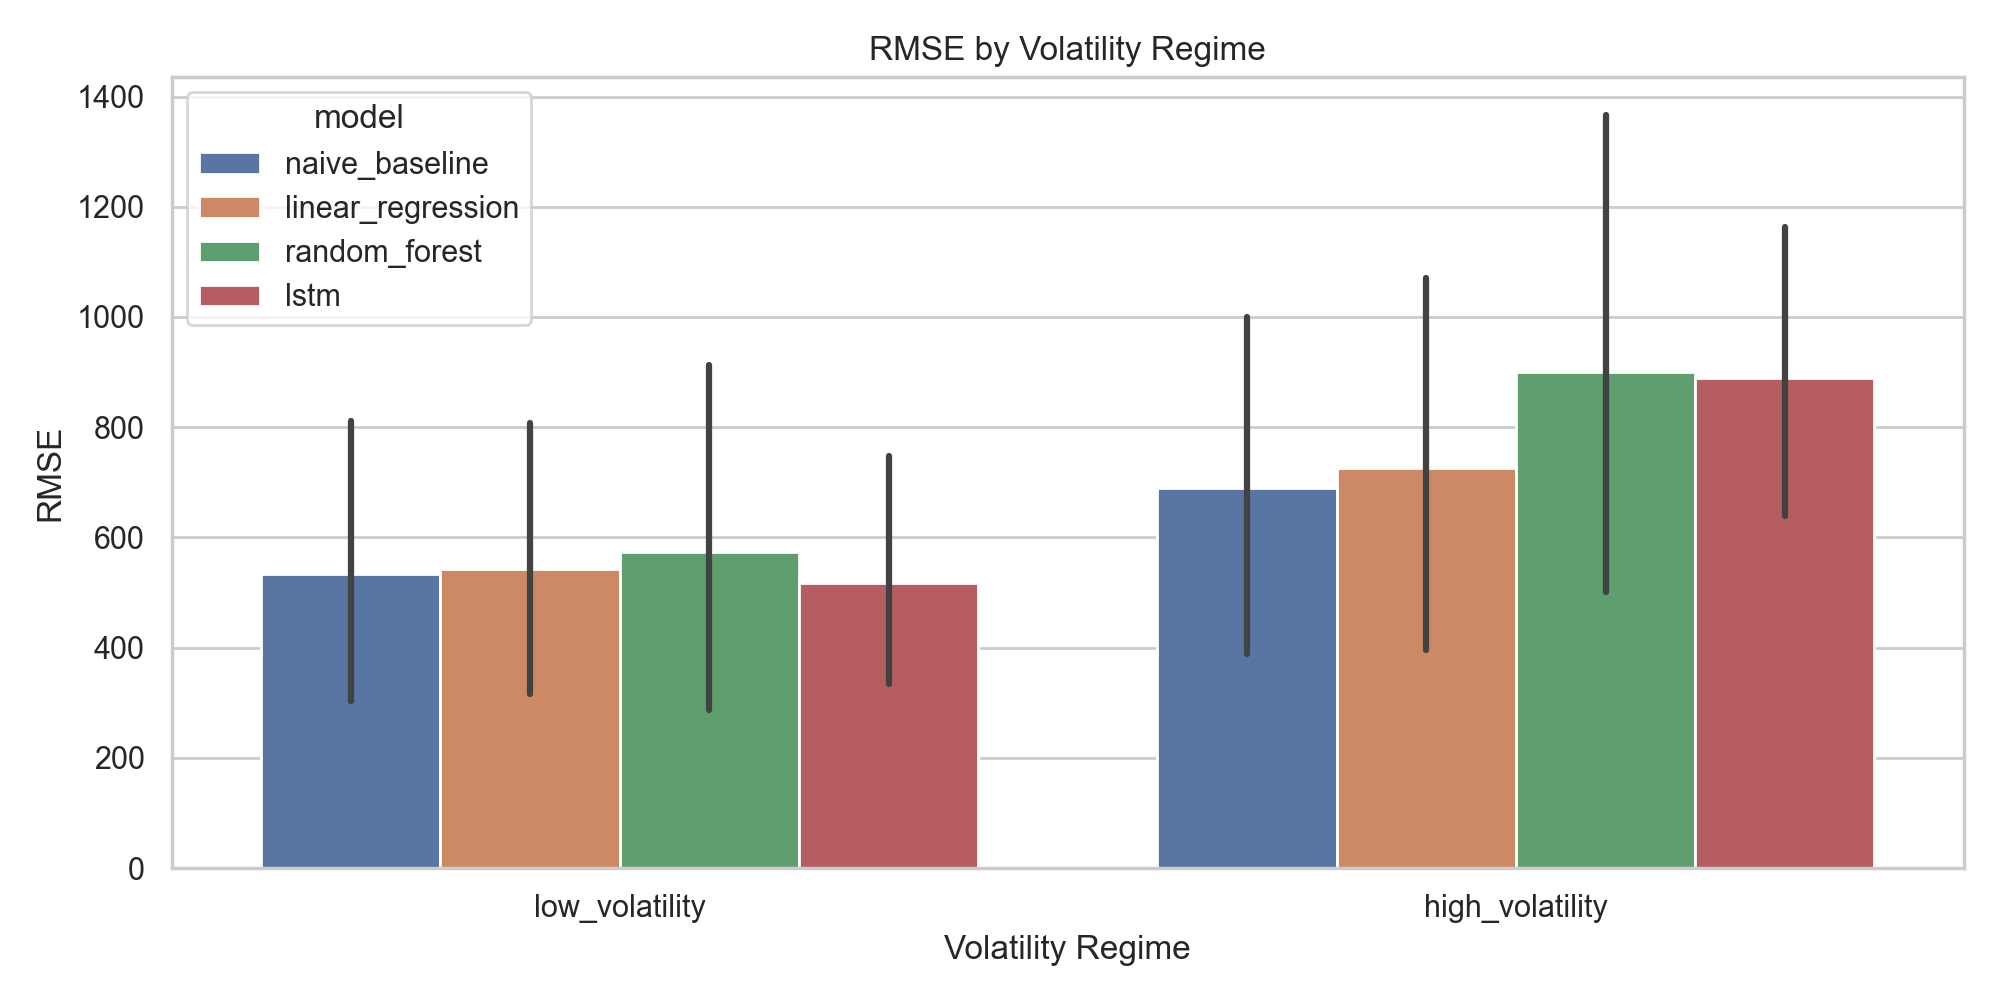
\includegraphics[width=\columnwidth]{../outputs/figures/rmse_by_regime.png}
\caption{RMSE comparison under low- and high-volatility test conditions.}
\label{fig:regime}
\end{figure}

Finally, Figure~\ref{fig:bestpred} plots actual versus predicted values for the best aggregate model setting, which is the one-day naive baseline. The predicted series closely follows the level of the actual series, but it still lags during rapid changes. This behavior is consistent with the persistence mechanism of the model itself.

\begin{figure}[!b]
\centering
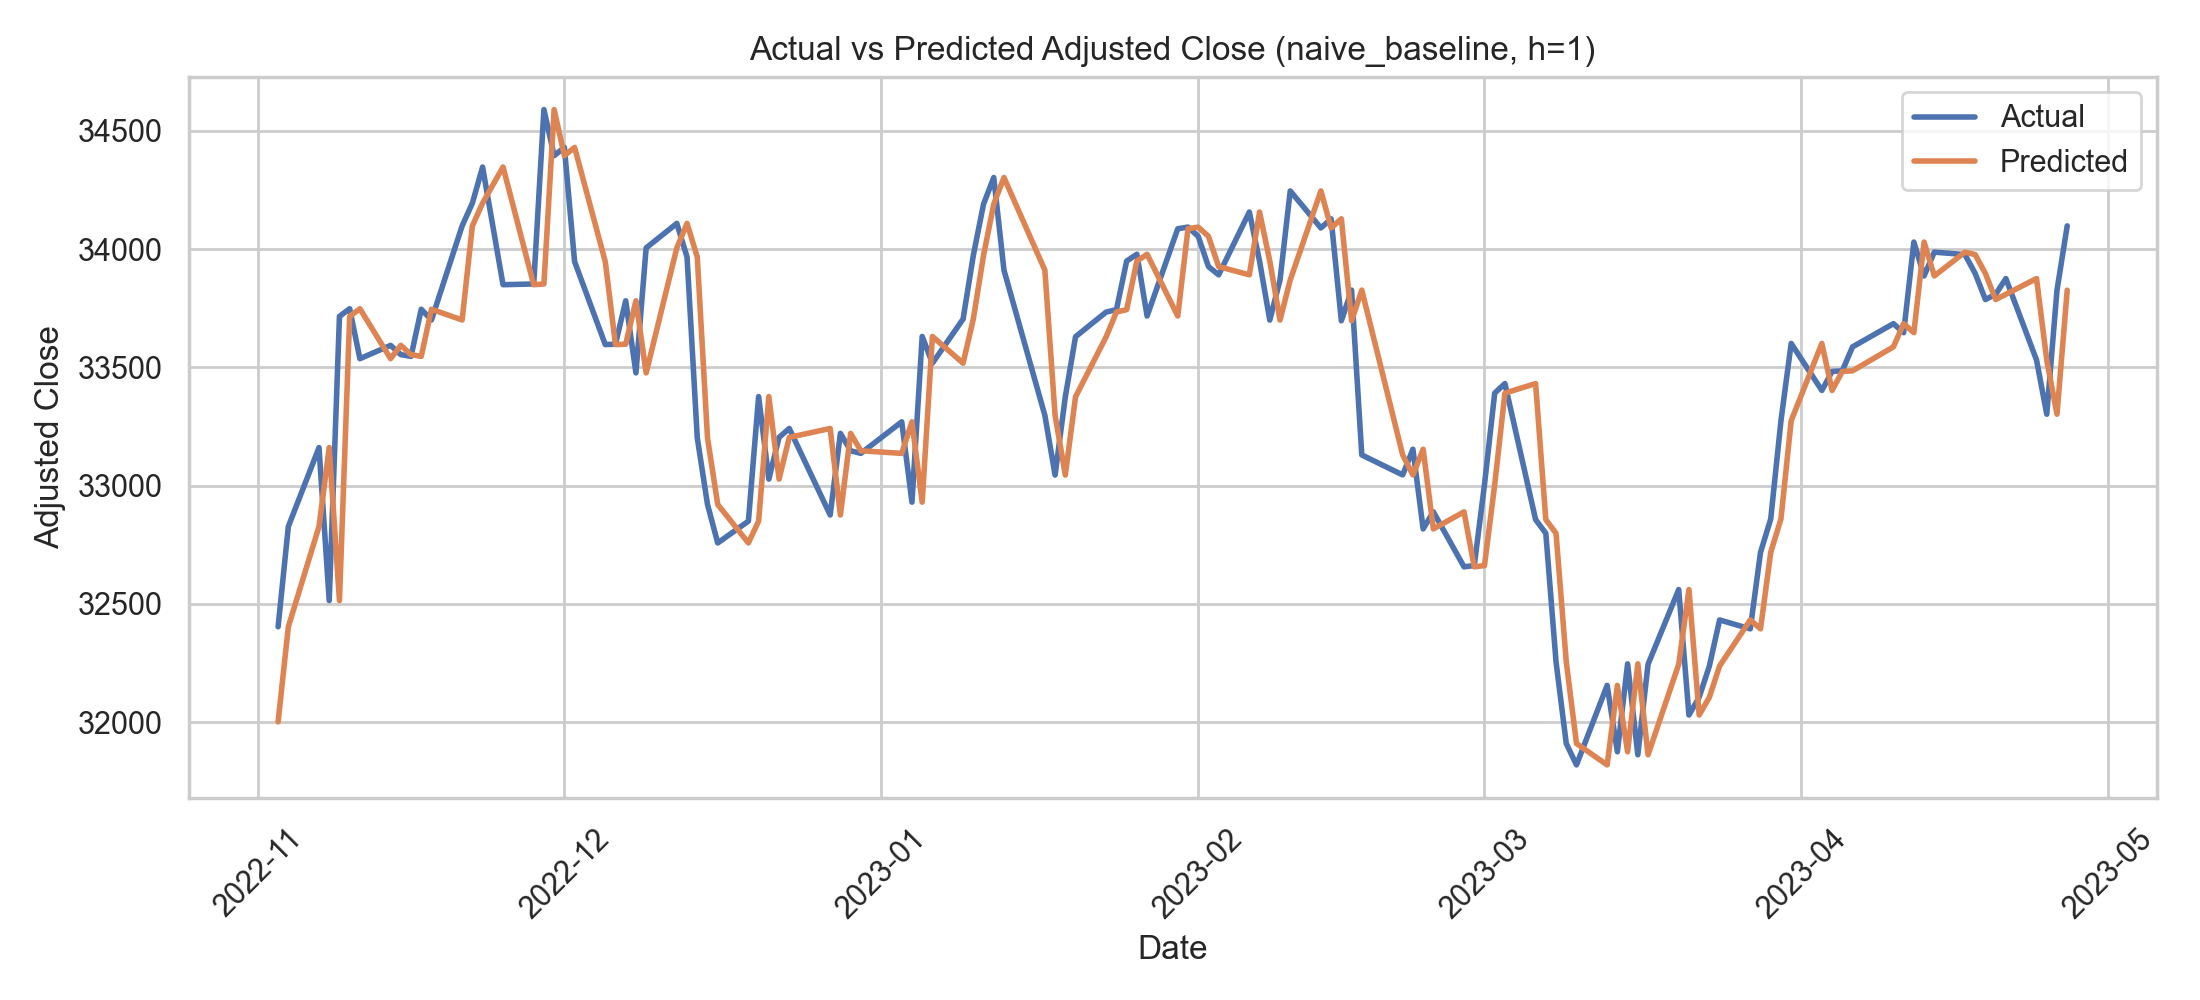
\includegraphics[width=\columnwidth]{../outputs/figures/best_model_predictions.png}
\caption{Actual versus predicted adjusted close for the best aggregate setting.}
\label{fig:bestpred}
\end{figure}

\section{Conclusion}
This project compared four forecasting approaches across multiple prediction horizons and volatility regimes using a daily Yahoo Finance time series from 2018 to 2023. Three main findings emerge. First, forecast error increases materially as the horizon expands from one day to seven days. Second, the naive persistence baseline outperforms the more complex models on the full test set at every horizon. Third, volatility strongly degrades predictive accuracy, and high-volatility periods are consistently the hardest to forecast.

At the same time, the regime analysis shows that model complexity is not uniformly useless. In low-volatility subsets, random forest and LSTM achieve the best RMSE for some horizons, although these findings should be read as suggestive rather than definitive because the low-volatility sample is small. The tuning stage also shows that the random forest underperformance is not simply due to an arbitrary default parameter choice. Even after selecting hyperparameters on the validation set, the tuned random forest remains weaker than the naive and linear baselines on the aggregate test set. The overall underperformance of the LSTM likely reflects the limited dataset size, the use of a single series, and the relatively simple architecture used here.

This project has several limitations. It uses one daily price series rather than a broad cross-sectional universe, relies on handcrafted features instead of richer macro or technical indicators, and predicts price levels rather than returns or directional movement. The tuning stage was intentionally lightweight rather than exhaustive, so future work could test broader hyperparameter searches, return-based targets, cross-asset features, and rolling-window retraining. Even with these limitations, the study demonstrates a complete Python forecasting pipeline and provides a clear empirical answer: in this dataset, short-horizon persistence is difficult to beat, and volatility is a central determinant of forecasting error.

\bibliographystyle{IEEEtran}
\bibliography{references}

\end{document}
